\chapter{Areas of Known Importance}\label{subsec:areasofknownimportance}
\subsection*{Why you need these maps} 
The Hudson River Valley has some of the greatest biodiversity in New York, 
owing to the combination of woodlands, wetlands, river, and mountain 
environments. Mature deciduous forests support an abundance of bird species as 
well as mammals, including black bear and bobcat. Streams and wetlands support 
fauna as diverse as river otter and native clams. \textbf{A 
prerequisite for making ecologically informed decisions about land use is 
knowing the types and locations of ecologically significant habitats within the 
town.} A ``habitat'' is a place where a particular species or group of species 
is likely to occur. The location and size of habitats relative to one another 
are also important to map as some habitats will not function in isolation or 
below a certain size threshold. These two maps should be consulted for land-use 
and development planning as a first step in identifying potentially significant 
habitats. This can inform planning and development in ways that minimize 
habitat degradation or loss.

\subsection*{Areas of Known Importance Map}\label{subsec:aokimportancemap}
This map shows areas of known importance for wildlife and plant habitats in the
Town of Cornwall and Village of Cornwall-on-Hudson based on information from
the \gls{nysdec} \gls{nynhp} inventory of rare species and migratory fish runs
and the Audubon \gls{iba} Program. Areas of Known Importance are defined as
lands and waters that support the continued presence and quality of known
populations of rare animals and rare plants, or of documented examples of rare
or high-quality ecological communities. In each case, these areas of importance
are tied to a recorded occurrence of that plant or animal and include areas
that support the natural ecological processes critical to maintaining the
habitats of these rare animal and plant populations, or critical to maintaining
these significant communities. Due to the potentially sensitive nature of this
information, exact locations and species are not shown. 
\paragraph{Rare Animals:} The areas of known importance for rare animals seen
on this map are tied to known occurrences of rare animals listed in
Appendix~\ref{app:cornwallspecies}. Areas may be important to a particular
species for foraging, roosting, winter habitat, nesting, migration, and other
uses. The vast majority of Cornwall has been identified as an important area
for one or more of these rare animals. The areas of the town with the greatest
concentration of overlapping important areas for rare animals are Black Rock
Forest, the Moodna Creek, the Hudson River, Schunnemunk Mountain State Park,
and Storm King State Park.
\paragraph{\textit{Rare Plants:}} Occurrences of rare plants have been recorded 
in the general locations shown on the map. The corresponding areas of importance for
these plants are focused on Black Rock Forest, Schunnemunk State Park, the
Hudson River shoreline, and the mouth of the Moodna Creek at Kowawese Unique
Area. A table of rare plant species that have been recorded in Cornwall can be
found in Appendix~\ref{app:cornwallspecies}.
\paragraph{\textit{Migratory Fish:}} The Moodna Creek and other streams such as 
Woodbury Creek and Mineral Springs Brook that feed into it are Moodna Creek are 
important spawning areas for migratory fishes including alewife (\textit{Alosa 
pseudoharengus}), blueback herring (\textit{Alosa aestivalis}), bay anchovy 
(\textit{Anchoa mitchilli}), American eel (\textit{Anguilla rostrata}), 
Atlantic tomcod (\textit{Microgadus tomcod}), and striped bass (\textit{Morone 
saxatilis}). A substantial warmwater fish community also occurs in the lower 
portion of Moodna Creek throughout the year~\citep{nysdosmoodna}. 
\paragraph{\textit{Birds:}} Significant portions of the town, mostly centered 
on the large forested and preserved areas, lie within the Audubon Society's 
\gls{iba}. In 2016, the Hudson Highlands West \gls{iba} was extended to include 
Black Rock Forest, Schunnemunk Mountain and the southern extension of the 
Schunnemunk Ridge, Woodcock Mountain (in the Town of Blooming Grove) and the 
surrounding areas. The Hudson Highlands West \gls{iba} defines an area of 
interior forest habitat that is critical for rare, threatened or endangered 
species or species on Audubon's watch list including the cerulean warbler, the 
wood thrush, and the blue-winged, worm-eating and prairie warblers. Black Rock 
Forest, where the most extensive records in the town have been kept, is home to 
over 150 species of birds, about two dozen of which are considered threatened. 
A catalogue of these species can be found 
\href{http://blackrockforest.org/files/blackrock/content/brf\_bird\_checklist\_current
\_for\_web\_0.pdf}{here}. 
\subsection*{Significant Natural Communities \& Biodiversity Areas}~\footnote{The 
Areas of Known Importance map~\ref{map:areasofknownimportance} shows data only 
from locations where surveys have been conducted. A systematic survey of natural 
communities or biodiversity is not available at a scale that is appropriate for 
this inventory. If such a survey existed, we would be likely to find other 
locations within the Town with significant natural communities and/or areas of 
high biodiversity. Therefore, the areas shown on these maps should not be 
considered to be the only areas that are important for biodiversity within the 
Town and Village. Field verification of habitats and their boundaries should be 
conducted prior to decision-making} \textit{Significant Natural Communities} are 
defined by the \gls{nysdec} \gls{nynhp} as locations of rare or high-quality 
wetlands, forests, grasslands, ponds, streams, and other types of habitats, 
ecosystems, and ecological areas. The \gls{nynhp} documents only those locations 
of natural communities where the community type is rare in New York State; or, 
for more common community types, where the community at that location is a 
high-quality example and meets specific, documented criteria for state 
significance in terms of size, undisturbed and intact condition, and the quality 
of the surrounding landscape.
\par
As the map indicates, the Town of Cornwall and the Village of
Cornwall-on-Hudson are home to a number of natural communities of state-wide
significance. These communities have been identified in the large protected
areas within the town's borders, including Schunnemunk State Park, Black Rock
Forest, and Storm King State Park. More detail on the communities shown on this
map can be found in~\ref{app:cornwallspecies}. 

\textit{\gls{sba}} are areas that contain high concentrations of biological diversity or
unusual ecological features that contribute to and serve as a framework for
conservation partnerships and voluntary protection efforts~\citep{haeckel2014}.
\gls{sba}s are defined by unique topography, geology, hydrology, and biology
that distinguish them from neighboring areas. \gls{sba}s carry no regulatory
designation. Instead, it is hoped that recognition of these areas will serve as
a basis for their voluntary conservation through conservation partnerships
involving multiple stakeholders.

Parts of the Town of Cornwall and the Village of Cornwall-on-Hudson lie within
two \gls{sba}s identified in the Hudson River Estuary Corridor: Hudson
Highlands and Mid-Hudson River~\citep{penhollow2006}.
\paragraph{\textit{Hudson Highlands Significant Biodiversity Area}}51\% of the 
Town of Cornwall is in the Hudson Highlands (West) Significant Biodiversity 
Area encompassing portions of Black Rock Forest (quadrants C, D, / 3, 4), 
Schunnemunk State Park (quadrants A, B / 3, 4), Schunnemunk Mountain Preserve 
(quadrants B3), and Storm King State Park (quadrants D, E / 2, 3). 55\% of the 
Village of Cornwall on Hudson is within the Hudson Highlands West Biodiversity 
area encompassing Roe Park and Donahue Memorial Park (quadrants D2). 

\paragraph{\textit{Mid-Hudson River Significant Biodiversity Area:}} Although not 
shown on this map, this area includes the Hudson River itself, and the lower 
portion of the Moodna Creek. 3\% of the Town of Cornwall (quadrants D, E / 1, 
2), and 2\% of the Village of Cornwall-on-Hudson are in the Mid-Hudson River 
\gls{sba}.

\includepdf[pages=-,fitpaper]{cornwall_maps/AreasofKnownImportance.pdf}\label{map:aok}
\namedlabel{map:areasofknownimportance}{Areas of Known Importance}
\chapter{Terrestrial Habitats}\label{subsec:terrestrialhabitats}
\subsection*{Why you need this map}
A habitat is a type of natural environment which provides conditions necessary 
for specific plants and animal species to live. Some major factors that 
contribute to terrestrial habitats are temperature range, amount of sunlight, 
moisture and precipitation levels, soil conditions, and the presence of food 
and predators. Flora and fauna species are specifically adapted towards certain 
habitats with varying degrees of specificity and range. Healthy, intact natural 
habitats support greater biodiversity, and major changes to those habitats can 
and do have unintended ecological consequences.
\par
Human influence on the landscape can create unique habitats that favor certain
species over others due to their relative adaptability. Agricultural
monocultures and human development can fracture the natural habitats of
migratory animals and large mammals, creating isolated “habitat islands” where
genetic diversity diminishes, and healthy populations of species become less
viable. Conversely, relatively intact and healthy habitats support species
diversity that can provide concrete benefits to a community. Bats control
insect populations. Bees and other pollinators are vital for agriculture,
coyotes help control the deer and rodent populations, and black and turkey
vultures eliminate carrion. The benefits of these species in turn help regulate
the habitats they function within and maintain a proper ecological balance for
a community. \textbf{Knowing the location of different habitat types or the preferred
habitats of endangered, threatened, or rare species can help prioritize
conservation of those habitats and protect the existing population of those
species.}
\subsection*{Habitats and Endangered Species}
If a species is endangered, it might be listed and therefore protected by the
\gls{esa}. A proposed project that is adjacent to or directly in an endangered
species’ habitat will likely need to be modified in order to accommodate these
species and minimize the impact to their habitat. Significant time may be
needed to work with the US Fish and Wildlife Service and other federal agencies
to design the project to minimize what is known as “taking.” The \gls{esa}
defines a ``taking'' as any of the following activities: harass, harm, pursue,
hunt, shoot, wound, kill, trap, capture, or collect any threatened or
endangered species. According to the \gls{nysdec}, there are currently six
wildlife species classified as endangered at the federal or state level that
have been identified in the Town of Cornwall. The species are: Golden Eagle,
Peregrine Falcon, Atlantic Sturgeon, Shortnose Sturgeon, Bog Turtle, and
Indiana Bat. Many other plant and animal species present in our Town such as
the Timber Rattlesnake are classified as threatened. It is important to note
that the health of terrestrial habits directly impacts the health of aquatic
habitats through the regional watersheds and aquifers that drain into major
regional creeks like the Moodna and ultimately the Hudson River. 

\subsection*{Habitats and Invasive Species}
Invasive species will often use the absence of natural predators to thrive and
spread much more aggressively than their native counterparts. This, in turn,
can create an imbalance in a habitat and threaten other species that rely on
native sources of food and shelter. The spread of non-native and invasive
species can also be a sign that a habitat is not in good health and is being
impacted by human influence or changes in climate factors such as temperature
or precipitation. One common way habitats are damaged is when increases in
certain nutrients, such as nitrogen from the application of fertilizers to
farmland, lawns, and golf courses, are outside the normal range for a
particular habitat. The overabundance of certain species like algae and other
plants are often a sign of point source pollution. Having up-to-date habitat
maps for a municipality can help track the habitat’s evolution, give an
indication of its health, and help determine what measures, if any, need to be
taken to mitigate damage from invasives and pollutants.
\par
\textbf{Healthy natural habitats are critical for hunters, hikers, and wildlife
enthusiasts, and, where threatened species like the bald eagle are concerned,
can often have a distinct cultural significance.} Municipalities can take steps
to reduce the impact of non-native species by providing recommendations for
native plants to residents, thus helping support healthier natural habitats. 

\includepdf[pages=-,fitpaper]{cornwall_maps/TerrestrialHabitats.pdf}\label{map:terrestrialhabitats}
\subsection*{Terrestrial Habitats Map}\label{subsec:terrestrialhabitatsmap}
\begin{itemize}
    \item The map clearly displays that forest habitats are the predominant
        habitat type within the town and village boundaries. Please refer to
        the~\nameref{map:forestpatches} Forest Patches and Regional Forest
        Linkage Zones map for more information about the importance of our
        forest habitats and tree cover.
    \item A general mix of hardwood and conifer growth and oak and pine specifically can be found
        throughout much of the town, earn more information and is especially
        concentrated in the preserved areas within Cornwall’s borders.
    \item Most of the cliff/talus habitat is located on the elevated terrain of 
         the two state parks within the town’s boarders: Storm King and Schunnemunk.
    \item Significant agricultural lands are found adjacent to the Moodna Creek to 
        the south and west of Interstate 87. Please refer to the~\nameref{map:meadowgrasslandsandshrublands} map for more information on the importance
        of both active and fallow agricultural habitats.
    \item The area around the mouth of the Moodna Creek and wetlands located on
        the southwest border of the town adjacent to Interstate 87 contain
        significant and important swamp hardwood habitats.
    \item Other significant
       mixed swamp habitats can be found in-between Interstate 87 and Stet Rt. 32
        towards the northern border of the town. Please refer to the~\nameref{subsec:wetland}
        narrative and the~\nameref{map:wetlandsandhydricsoils} for more
        information on the importance of these habitats
\end{itemize}
Note: In addition to generalized residential and commercial development, 
certain active and inactive railroad beds and paved and dirt roads are shown
as ``developed land'' on this map.

\chapter{Forests}\label{subsec:forests}
\subsection*{Why this habitat is important}
The value of trees and green spaces to a community is almost universally
understood. We all appreciate the shade, temperature moderation, and sense of
well-being that trees bring to our lives. What many may not realize, however,
is that patches of forest (both large and small) are also vital for providing
wildlife habitat, mitigating the effects of air pollution, filtering water that
drains into our aquifers and wells, and easing the increasing effects of
climate change. \textbf{Generally speaking, larger forests provide greater
ecological value than smaller, fragmented patches; however, the value of each
forest is relative to the values of other forests in the community, watershed,
or natural landscape.} Even small patches of forest can be extremely valuable
depending on different factors~\citep{haeckel2014}. If we look at the forest
that borders the Moodna Creek, we see an important wildlife corridor that
allows native species to move from one patch of forest to another. When we look
at the forested land that extends out beyond the borders of our state parks, we
see dense, deep-rooted growth that stabilizes our slopes and protects our homes
and businesses from flooding and damaging erosion.\\
In general terms, forested land provides a community the following benefits~\citep{bradfordcc}:
\begin{itemize}
    \item Protect watersheds and groundwater, holding soils in place and 
    reducing runoff, recharging aquifers, and supplying clean water to our 
    ponds, rivers, streams, and water supplies.
    \item Reduce flooding by slowing the release of storm water and snowmelt to downstream areas.
    \item Provide habitat and movement corridors for wildlife.
    \item Contribute to soil formation. 
    \item Mitigate the effects of extreme weather by cooling the air on hot summer days and reducing wind chill factors in the winter.
    \item Produce oxygen, capture carbon dioxide, and help clean the air of pollutants.
\end{itemize}
\subsection*{Forest Characteristics}\label{subsec:forestcharacteristics}
Many different types of forest can be found in the Hudson Valley Region.
Because our region is an important biome transitional zone between the
oak-hickory, northern hardwood, and boreal forest types, we have nearly ten
boreal and more than twenty southern temperate tree species living near or at a
range limit~\citep{ldeo}. This means that we have more species of trees than other regions
further to the north or south, and this forest biodiversity in turn supports
many important and iconic wildlife species such as black bear, wild turkey, and
numerous migratory song birds. These species are dependent on healthy, intact
forest patches to maintain their population.

To better quantify the ecological and commercial value of forested land, it is
important to designate its significance within the region.
\begin{itemize}
    \item \textit{Regionally significant forests} contribute to resiliency in a
        changing climate and have a high conservation value because of that
        function. Preserving these larger blocks of forest and the linkage zones that
        connect them will maintain wildlife corridors, reduce the impact of invasive
        species, and provide recreational benefits to areas experiencing growth in
        eco\-tourism. 
    \item \textit{Locally significant forest} blocks are equally important to 
        regulating temperature and controlling the effects of whether
        events, but often have reduced habitat value for wildlife. Areas where
        development has infringed on forest habitat often see a more limited
        capacity for forest regeneration due to a higher presence of invasive
        species and over browsing by deer among other factors. 
    \item \textit{stepping stone forest} is important because it provides a
        bridge between these larger patches of biodiverse forest and allows
        for the establishment of ecological networks or corridors that help
        lessen the fragmentation of forest habitat, maintain the integrity
        of migratory pathways, and generally increase the viability of
        plant and animal wildlife.
\end{itemize}

\subsection*{Forest Patches and Regional Linkage Zones Map}\label{subsec:forestpatchesandreglinkagezonesmap}
Because certain portions of Cornwall lie within the boundaries of two state
parks and the Black Rock Forest Consortium, our municipality’s overall forest
cover is considerable compared to others. This map shows the forest cover
within the borders of Black Rock Forest and on the adjacent land of West Point
to the south as regionally significant both for its size and the wildlife
habitat that it supports.
\begin{wrapfigure}{R}{7cm}
    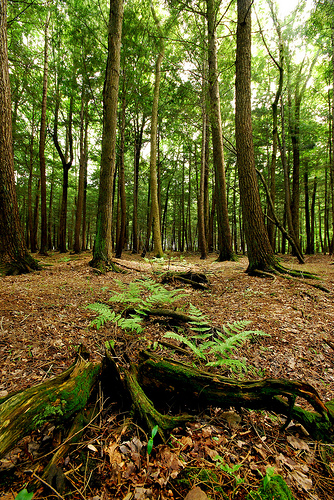
\includegraphics[width=6.85cm, keepaspectratio]{images/forest.jpg}
    \caption{\textit{North American Forest}\label{fig:forest}}
    %\vspace{-\baselineskip}
\end{wrapfigure}
Much of the village is classified as locally significant forest despite its
low-density residential development, and plays an important role in linking the
regionally significant forest patches to the river as well as providing a
buffer zone from more robust human development. The land protected by
Schunnemunk State Park is similarly classified as being locally significant and
is a reflection of the fact that continued development threatens to create a
habitat island, isolated from more biodiverse forest land.

Outside of these areas, the map identifies large parts of Cornwall as containing
stepping stone forest cover. The map also shows that most of these stepping
stone forest areas act as important regional linkage zones between locally and
regionally significant forest patches, and even combine with the regionally
significant forest of the Hudson Highlands to define the area between County
Rt. 32 and the southeastern border of the town as vital matrix forest (see
below). Of particular note in these stepping stone forest designations are
parts of Cornwall such as the land adjacent to state Rt. 9W and the Moodna
Creek that have been proposed for large scale residential development in the
past.
\includepdf[pages=-,fitpaper]{cornwall_maps/ForestPatchesRegionalForestLinkageZones.pdf}\label{map:forestpatches}

\chapter{Stream and Riparian Habitat}\label{subsec:streamandriparianhabitat}
\subsection*{Why you need this map}
We all have enjoyed, been impacted by, or taken actions that impact Cornwall's
stream and riparian habitats. Cornwall Elementary School at Lee Road students
learn about the riparian habitat of Black Rock Forest reservoirs during their
3-season scientific expeditions. Parents and grandparents enjoy teaching their
children and grandchildren how to fish at Ring’s Pond. Some children will
disappear for hours along our many streams, exploring the plants and animals
that call these habitats their home and cooling off on hot summer days. As the
frequency of heavy rainstorm has increased by 74\% since the 1950s, we have
also experienced the swelling of our streams beyond their channels to former
floodplains where we have built many of our homes and other structures. We may
have inadvertently exacerbated this situation by removing the vegetation that
not only protects the plants and wildlife in our watercourses, but also
protects our properties from these floodwaters.

Streams and streamside, or riparian, areas are important transitional zones
where land and water are linked~\citep{haeckel2014}. Streams include the banks,
floodplains, and non-floodplain areas next to streams. Streams, if healthy, can
support the plants and microhabitats of small aquatic animals that are
important to the survival of native fish, like brook trout, American eel, and
herring species. Additionally, streams are key in the life cycles many other
species, like mink, bats, belted kingfisher, herons, wood turtles, stream
salamanders, and dragon flies by providing food and areas for breeding,
migration, hibernation, and safety.~\ref{app:cornwallspecies}
provides a comprehensive listing of species of conservation concern. Retaining
current floodplains supports habitats that can withstand occasional flooding,
such as meadows, swamp, marsh, and lowland forest, thereby supporting the
animals that rely on these habitats and other animals that rely on them for
food~\citep{haeckel2014}.

Maintaining the health of stream and riparian habitats involves the retention
and addition of native trees for shading to keep streams cool for our coldwater
fish, brook trout. The retention and addition of native shrubs, grasses, and
wildflowers can protect animal life by preventing unwanted vegetation,
sedimentation, and pollution reaching our streams and waterbodies as well as
reduce the impact of flooding. Orange County Water Authority's
\href{https://www.orangecountygov.com/DocumentCenter/View/4135/Watershed-Design-Guide-2014-PDF}
{Watershed Design Guide} provides a comprehensive visual explanation of healthy
streamside plantings based on the recommendations detailed in its
\href{https://www.orangecountygov.com/DocumentCenter/View/4133/Moodna-Creek-Watershed-Conservation-and-Management-Plan-2010-PDF}{Moodna Creek Watershed Conservation and Management Plan}
The Upper Esopus Creek Management Plan Newsletter of Cornell University Cooperative 
Extension Ulster County provides sample native streamside plantings for our 
neighbor to the north, Ulster County.

\subsection*{Town of Cornwall and Village of Cornwall-on-Hudson}
\subsection*{Stream Classification Map}
%(hyperlink to that section in the narrative)
This map informs us of the existing or best uses of our local streams as well
as their quality and purity. According to the 2017 \gls{nysdec} data, many
streams in the Town are suitable trout habitat, with some suitable for trout
spawning, or release of eggs.

\subsection*{Stream Biomonitoring and Priority Waterbodies Map}
Notable on this map are the many dams and culverts that pepper our streams.
Culverts, if properly installed, can foster the natural life cycles of trout
and American eel, for example, by allowing them to travel upstream. While
long-standing dams have created much-appreciated features such as lakes and
ponds, it is now understood that they also play a role in isolating and
severely limiting the range of aquatic species and other organisms that use
stream corridors as well as a role in increasing local flooding and
deteriorating water quality~\citep{haeckel2014}.
%(hyperlink to that section in the narrative)
%Good location for image of culvert 

\chapter{Wetland Habitat}
\subsection*{Why you need this map}
Wetland habitats serve two very important roles: they are key to the survival
of many species while providing flood-control and water cleansing benefits for
Town and Village communities. Wetland habitats come in many different forms and
support many different types of species. They include wet clay meadows,
hardwood swamps, emergent marches, and vernal pools. According to
\gls{nysdec}'s~\ref{app:cornwallspecies}, our wetlands are home to the following
animals and plants that are threatened, of special concern, or of greatest
conservation need: Least Bittern, Common Snapping Turtle, Northern Copperhead,
Marbled Salamander, Clustered Sedge, and Large Twayblade.
\href{https://ecode360.com/10555547?highlight=wetlands#10555547}{Chapter 90
Freshwater Wetlands} of the Town’s Code provides a comprehensive listing of the
vegetation that is associated with seasonal or permanently flooded wetlands.
Beavers, muskrats, and dragon flies are just a few of the additional animals
for which wetlands are important.

Vernal pools are of particular interest because they are typically small in
size and not well documented. These seasonal woodland pools don't always
support wetland vegetation, but they are critical breeding habitat for several
species of forest salamanders and frogs, such as spring
peepers~\citep{haeckel2014}. A wetland ground-truthing exercise would be
instrumental to identifying not only seasonal wetlands, but also smaller
wetland habitats that are not captured by the various data sources for the~\nameref{map:wetlandsandhydricsoils}.
See section~\nameref{subsec:wetland} for more information.

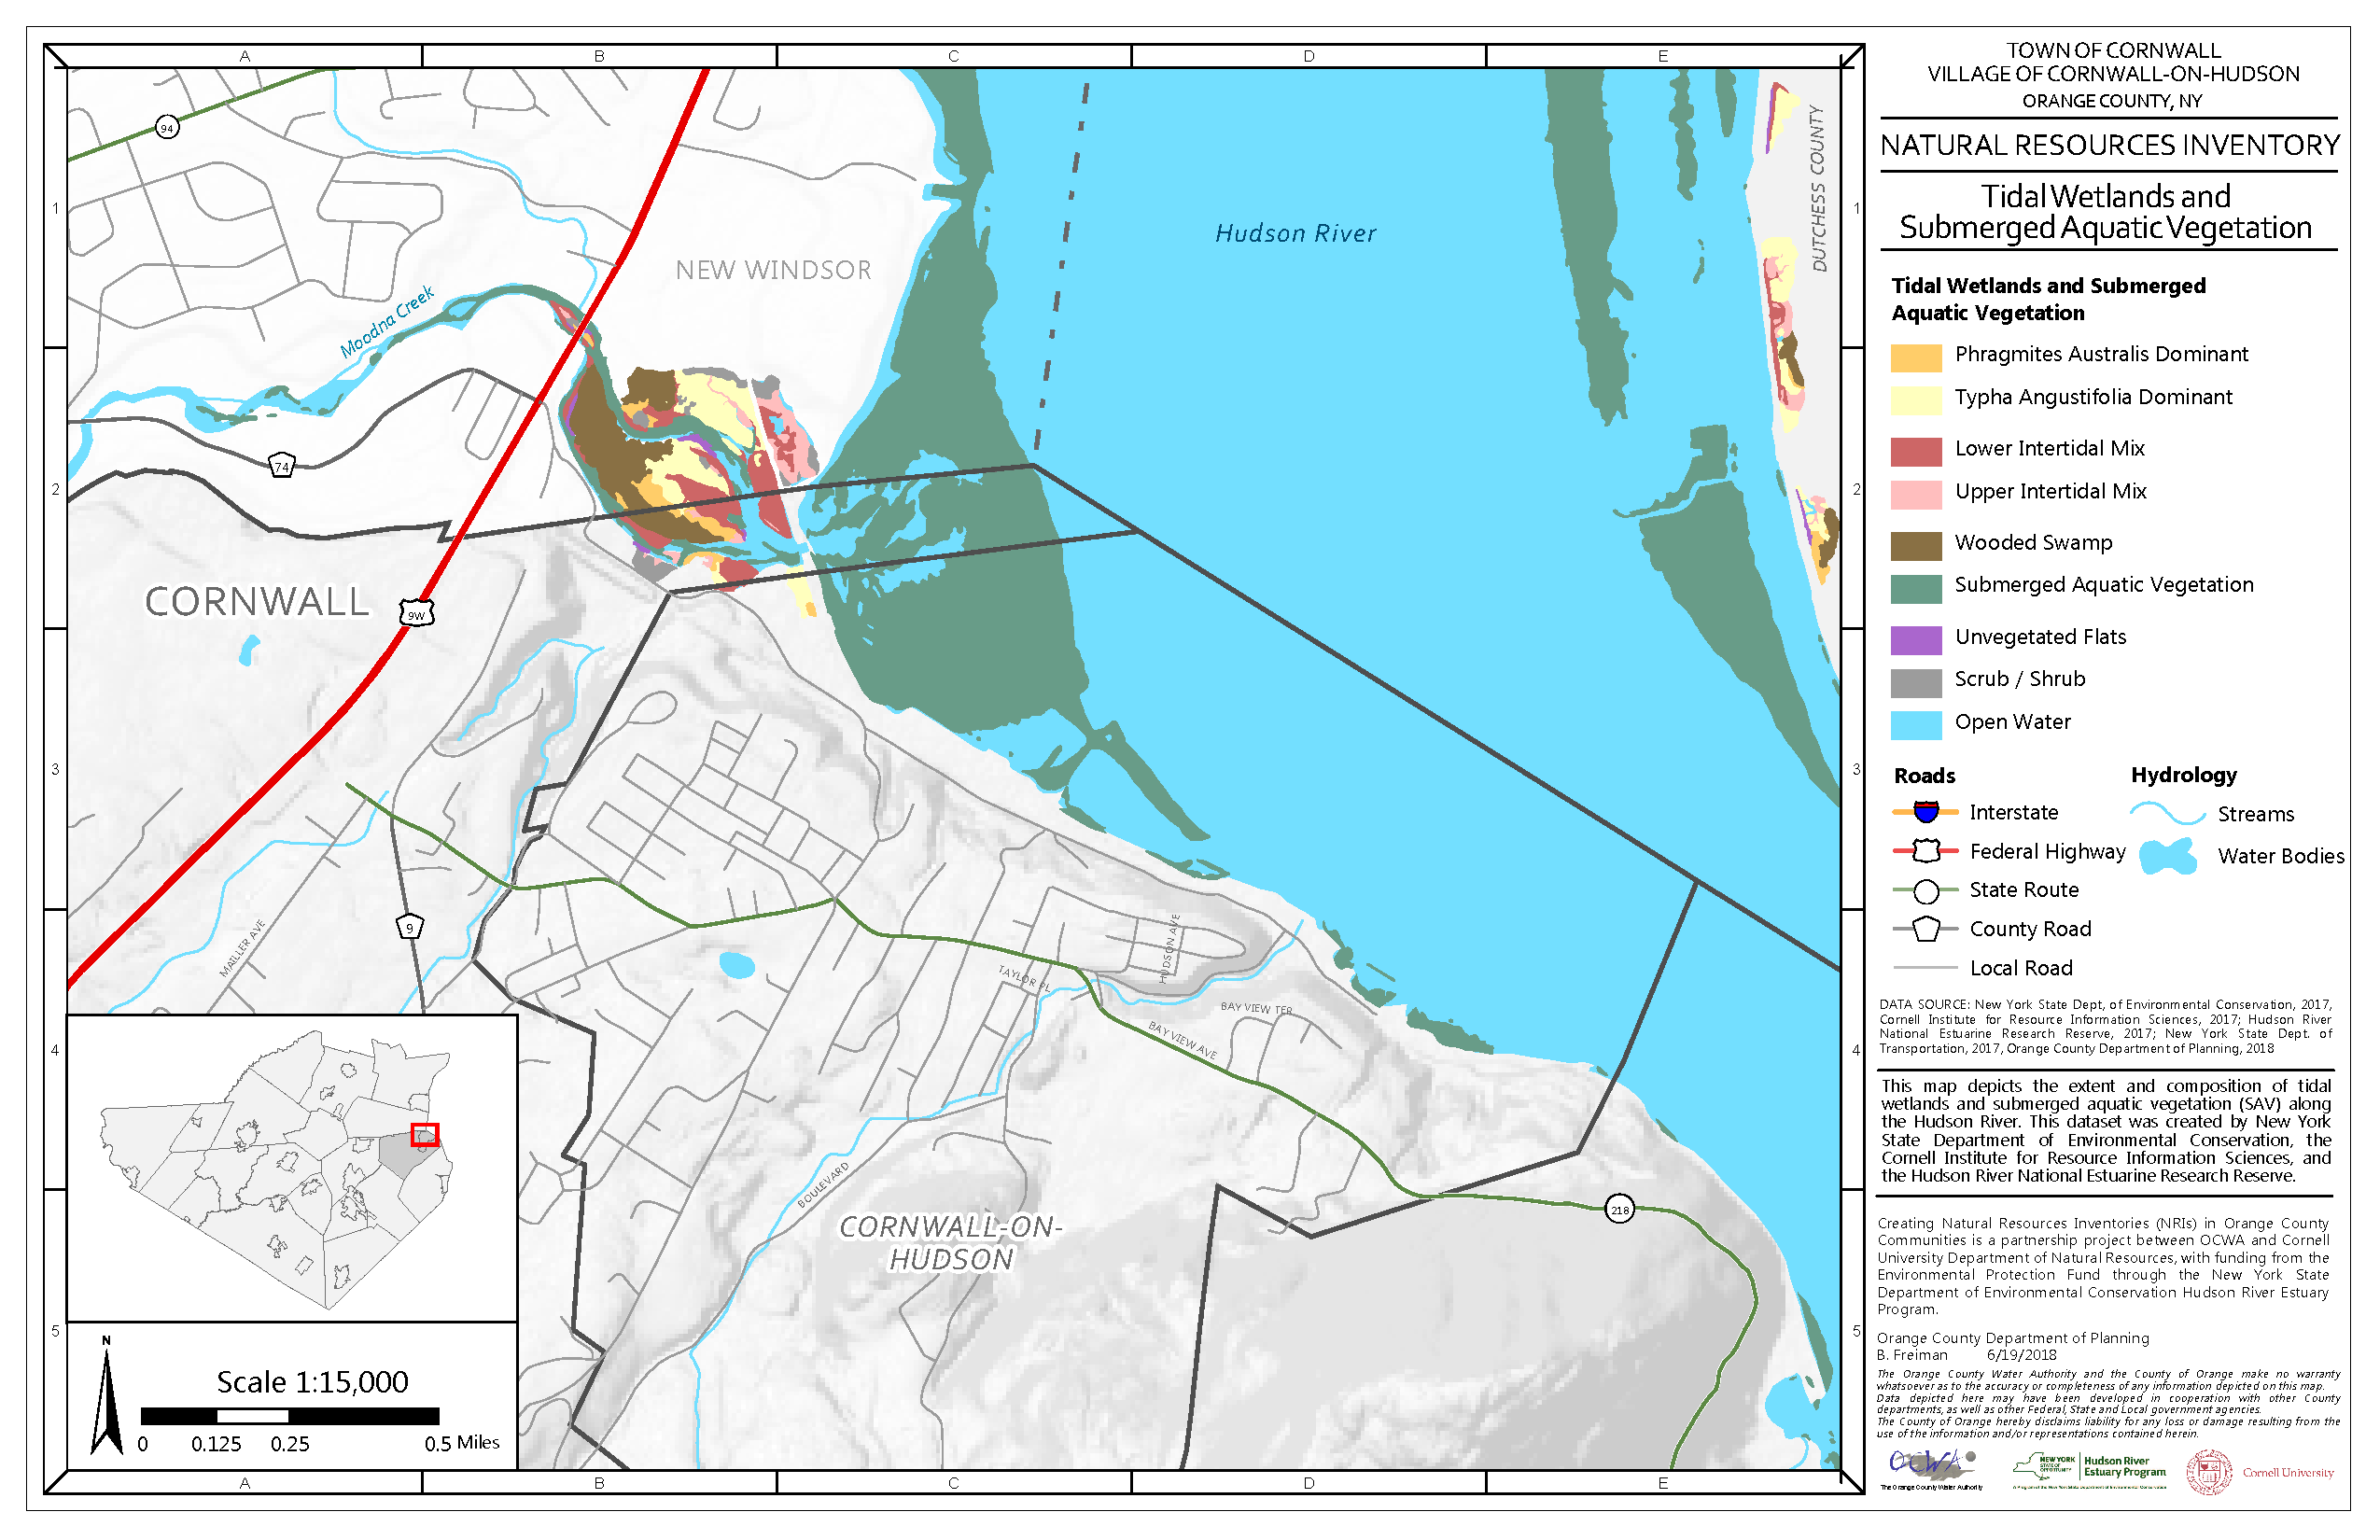
\includepdf[pages=-,fitpaper]{cornwall_maps/TidalWetlandsandSAV.pdf}\label{map:tidalwetlandsandSAV}
\chapter{Tidal Wetland Habitat}\label{subsec:tidalandwetlandhabitat}
Tidal wetlands are some of the most important habitats within the Hudson River
Estuary. They support numerous unique species that rely on the changing water
level to survive, and that are especially suited for that habitat type. Tidal
wetlands and \gls{sav} not only support a great diversity of plant, animal, and
insect life, they also contribute to the economic significance of the estuary.

\begin{wrapfigure}{R}{7cm}
    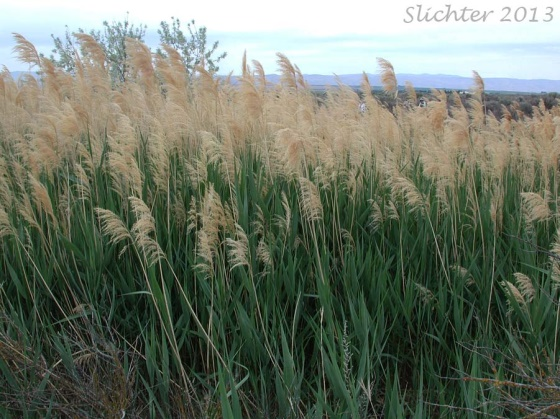
\includegraphics[width=6.85cm,keepaspectratio]{images/Common_reed.jpg}
    \vspace{-5pt}
  \caption{\textit{Phragmites australis}}
\end{wrapfigure}
\begin{displayquote}
More than 200 species of fish are found in the Hudson, including key commercial
and recreational species like striped bass, and species of conservation
concern like Atlantic and short-nose sturgeon. \gls{sav} beds improve water
quality in the Hudson and provide essential habitat for invertebrate
animals, which feed fish and waterfowl that use the estuary. Tidal wetland
habitats play a critical role as nursery grounds for fish and shellfish
species, as well as providing nesting sites and migration stops for birds
and sources of nutrients for the estuary food web. These wetland systems
also help filter pollutants, buffer shoreline properties, and help
stabilize the river’s shoreline~\cite{haeckel2014}.
\end{displayquote}
Given the trend of sea level rise due to climate change, \textbf{it is also
important to note that tidal wetlands can help reduce flooding by limiting wave
action and acting as an intermediate habitat between the land and the water.}
They are often great places for recreation, providing opportunities for fishing
exploring by kayak or canoe. 
Since tidal wetlands are extremely dynamic systems, they are constantly
changing. However, long term changes can be seen in vegetation type and
sediment levels. Many wetlands have been invaded by the common reed
(\textit{Phragmites australis}). Areas with native cattail (\textit{Typha
angustifolia}) tend to be much more biologically diverse than areas invaded by
Phragmites, and more biodiversity in the plant community can increase the types
of other animals that use a given area for shelter or food. As the climate
changes and sea level rises, water levels may increase faster than wetlands can
gain new sediment, which could cause decreased amounts of these crucial
habitats for plants and animals~\citep{nysdectidal}. 
\gls{sav} provides important habitat for juvenile fish that can hide within the
leaves. In addition to fish, \gls{sav} beds provide habitat for
macroinvertebrates, and food for waterfowl, either by eating the plants
themselves or eating the animals living in the plant beds. \textbf{\gls{sav} is
an important source of oxygen in the water, which aquatic animals need to
survive and is used as a key measure of water quality.} Water celery is the
most common native submerged aquatic plant in the Hudson River. A very common
invasive species impacting \gls{sav} is water chestnut (\textit{Trapa natans}),
which can be seen in almost every freshwater, slow moving area of the Hudson
River in the summertime. Water chestnut creates mats of leaves at the surface
of the water, shading out native water celery below. The water underneath water
chestnut beds are known to have much lower oxygen levels than other areas.
While water chestnut does produce oxygen, they release it into the air through
their leaves floating at the top of the water, instead of directly into the
water like other aquatic plants would~\citep{nysdecsav}.
\begin{wrapfigure}{L}{7cm}
    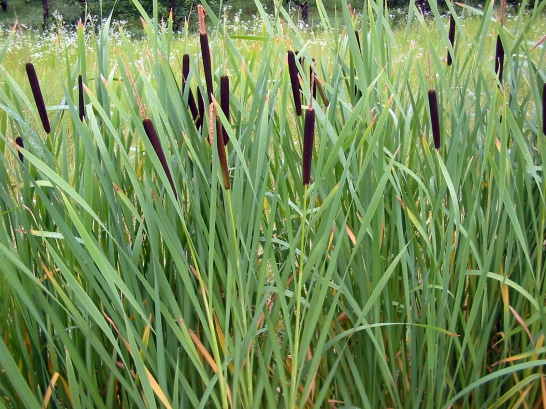
\includegraphics[width=6.85cm,keepaspectratio]{images/Cattail.jpg}
    %\vspace{-10pt}
    \caption{\textit{Typha angustifolia}}
\end{wrapfigure}

\textbf{Although these habitats support extraordinary biological diversity and
provide important benefits to humans, they have been diminished, damaged and
disconnected by human patterns of development during the last 150 years.} Vast
areas of river bottom have been dredged to create and maintain a shipping
channel. Tidal wetlands and shallows have been filled, and, in some areas, fill
covers a third of the river's original surface area. Nearly half the Hudson's
shoreline has been straightened and hardened by human-made structures.
Compounding these losses are impacts from sea-level rise and climate change
which threaten shoreline and shore communities where water may rise faster than
habitats can build up sediments to keep pace. Also, human responses to
sea-level rise and increased flooding may include building dikes which will
prevent habitats from migrating landward. Finally, the ongoing accidental and
deliberate introduction of invasive plants and animals continues to threaten
native species and their habitats~\citep{nysdosmoodna, anderson2013}.

\begin{wrapfigure}{R}{8cm}
    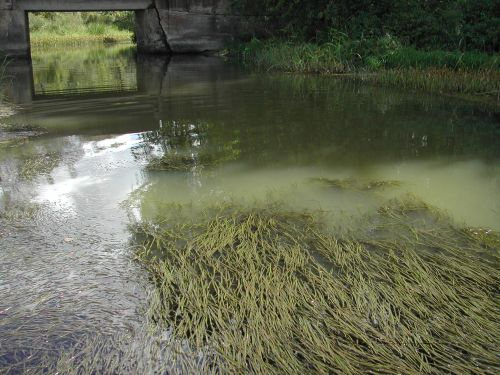
\includegraphics[width=7.6cm,keepaspectratio]{images/Water_Celery.jpg}
    \caption{\textit{Vallisneria americana}}
\end{wrapfigure}

\subsection*{Tidal Wetland Habitat}
Cornwall has only a small area of tidal wetlands, but that area, the mouth of
the Moodna Creek, is an important component in Cornwall’s contribution to the
overall health of the Hudson River estuary. The map shows the distribution of
the two primary tidal wetlands reed species common to the area, \textit{Typha
angustifolia} (native) in yellow and Phragmites australis (invasive) in orange.
Also shown are wooded areas (brown), barren areas and mud flats (purple), and
areas of upper and lower intertidal mixed vegetation (pink and red,
respectively).

To the east of the Moodna outlet is a large area of submerged aquatic vegetation 
(dark green). This \gls{sav} growth follows along much of the shore line of the 
town and village with the exception locations where development has occurred and 
hardened shoreline has been created (i.e.; Donahue Park). gls{sav} is also 
present through most of the Moodna creek outlet and runs approximately 2/3 of a 
mile up the creek itself in patches. All of this \gls{sav} provides important 
nursery habitat for numerous fish and wildlife species.

\chapter{Grasslands and Shrublands}\label{subsec:grasslandsandshrublands}
\subsection*{Why this habitat is important}
\begin{wrapfigure}{L}{10.5cm}
    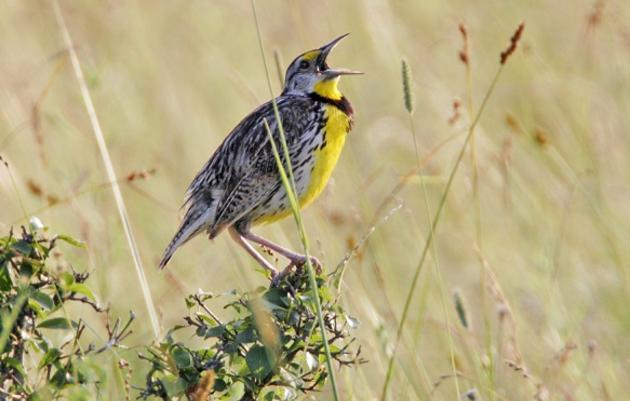
\includegraphics[width=10.38cm, keepaspectratio]{images/bird.jpg}
  \caption{A bird}
\end{wrapfigure}
Meadows, grasslands, and shrublands are unique and valuable habitats that are
critical for bird, plant, and wildlife communities. Historically, Native
peoples, fires, and beaver were the primary forces responsible for creating and
maintaining grassland and meadow habitats in New York. Native Americans created
grasslands when they burned the land for agriculture and to improve forage for
game species such as white-tailed deer. At the same time, ponds above abandoned
beaver dams grew into grassy meadows after the water drained and the
nutrient-rich soil was exposed to sunlight. In more recent history, fire
suppression and limits to where beavers are allowed to build dams has meant
that grass and shrublands are restricted mainly to agricultural areas. The peak
of agricultural clearing in the northeastern US occurred in the
mid-1800s~\citep{unhextension} Since then, \textbf{the amount of land
identified as grassland or shrubland has decreased rapidly in the
Northeastern United States}. This is mostly due to increases in population and
resulting development, and changes in agriculture that has resulted in the
abandonment of many small, family-owned farms. Unused farm land has
traditionally been a major target for sale and development and is typically one
of the first habitats to succumb to low-density residential development.

Native wildflower growth in these habitats is a vital source of support to
pollinators, and numerous species depend on open grassland and shrubland
habitats, especially grassland breeding birds that require large meadows for
successful nesting. New York State's grasslands are home to significant
populations of some of the highest priority birds in the Atlantic Flyway. These
birds, which have been sentinels of environmental health for centuries, depend
on hayfields, pastures, fallow fields, and other agricultural lands for
essential habitat. But the same bird species are experiencing significant
declines in populations. Scientists report a 90\% decrease in targeted
grassland species since 1966~\citep{audoboniba}. Some of these species such as Henslow's
Sparrow, Upland Sandpiper, Grasshopper Sparrow, Short-eared Owl, and Eastern
Meadowlark are area-dependent species, meaning that they need large unbroken
expanses of grasslands to thrive and reproduce. The amount of grassland habitat
needed by these species depends on factors such as location, shape, surrounding
habitats, and vegetative composition, however, as a general rule, grasslands
need to be at least twenty-five acres in size to offer appropriate habitat for
at-risk grassland birds in New York. The~\ref{map:areasofknownimportance}
map shows the extent of the Audubon Important Bird Areas that lie within the
borders of Cornwall.

Old farm fields or forest clearings are by nature transitional and relatively
short-lived habitats, usually quickly colonized by shrubs and requiring
periodic management to maintain openness. Shrublands in turn revert rapidly to
forest without continued maintenance or disturbance, such as fire, that
triggers young forest growth. Where they still occur, conserving and managing
large grasslands and shrublands benefits wildlife and can also support
agricultural land uses and scenic values~\citep{haeckel2014}.
\subsection*{Meadows, Grasslands, and Shrubland Map}
Cornwall is home to a considerable amount of meadow, grassland and shrubland.
Much of the town’s land that is not mountainous or developed falls into this
category. This map shows all of the significant parcels within the Town of
Cornwall and the Village of Cornwall-on-Hudson Cornwall ranked by acreage; the
lightest shading being small parcels of 10 or fewer acres, and the darker
shading denoting large parcels of more than 50 acres. Most of Cornwall's large
parcels of grasslands and shrublands are located in the west of the town,
clustered at the foot of Schunnemunk Mountain. Other significant parcels lie on
either side of State Route 94 and County Route 20 (Orrs Mills Road).

Cross referencing the~\nameref{map:landcover} under the land use section in
this NRI shows that the majority of these grasslands and shrublands are either
actively cultivated farmland or pasture, or preserved lands that were
previously cultivated and left as pasture. Looking at the~\ref{map:protectedopenspace}
map in the land use section, one can see that significant portions
of these preserved grasslands and pasture are now within the boundaries of
state parks, public nature preserves, museums, or conservation easements.
Because these lands are preserved and actively maintained, this ensures that
annual mowing occurs and keeps these parcels from becoming shrubland and
returning back to forested land. As noted above, this is important for
maintaining vital grassland bird habitat in the Hudson Valley.

While the Village of Cornwall-on-Hudson is heavily forested outside of its
central developed areas to the north, it does contain a number of grassland
parcels, the most significant being the former Donahue Farm parcel off of
Hudson Street. Privately owned and maintained land accounts for the other
significant grassland or shrubland parcels in the Village.
% 218?
\includepdf[pages=-,fitpaper]{cornwall_maps/MeadowsGrasslandsandShrublands.pdf}~\label{map:meadowgrasslandsandshrublands}
